\chapter{Hierarhično razvrščanje v skupine}
\label{ch:hierarhicno-razvrscanje}

Ena od nalog rudarjenja besedil je iskanje zanimivih skupin dokumentov. Torej radi bi odkrili dokumente, ki so si podobni mes sabo. 

Poglejmo si preproste podatke z dvema stolpcema (glejte opombo) in jih prikažimo v gradniku \textit{Scatter Plot}. Koliko skupin imamo? Kaj predstavlja različne skupine? Kateri primeri sodijo v posamezeno skupino?

\begin{figure*}[h]
    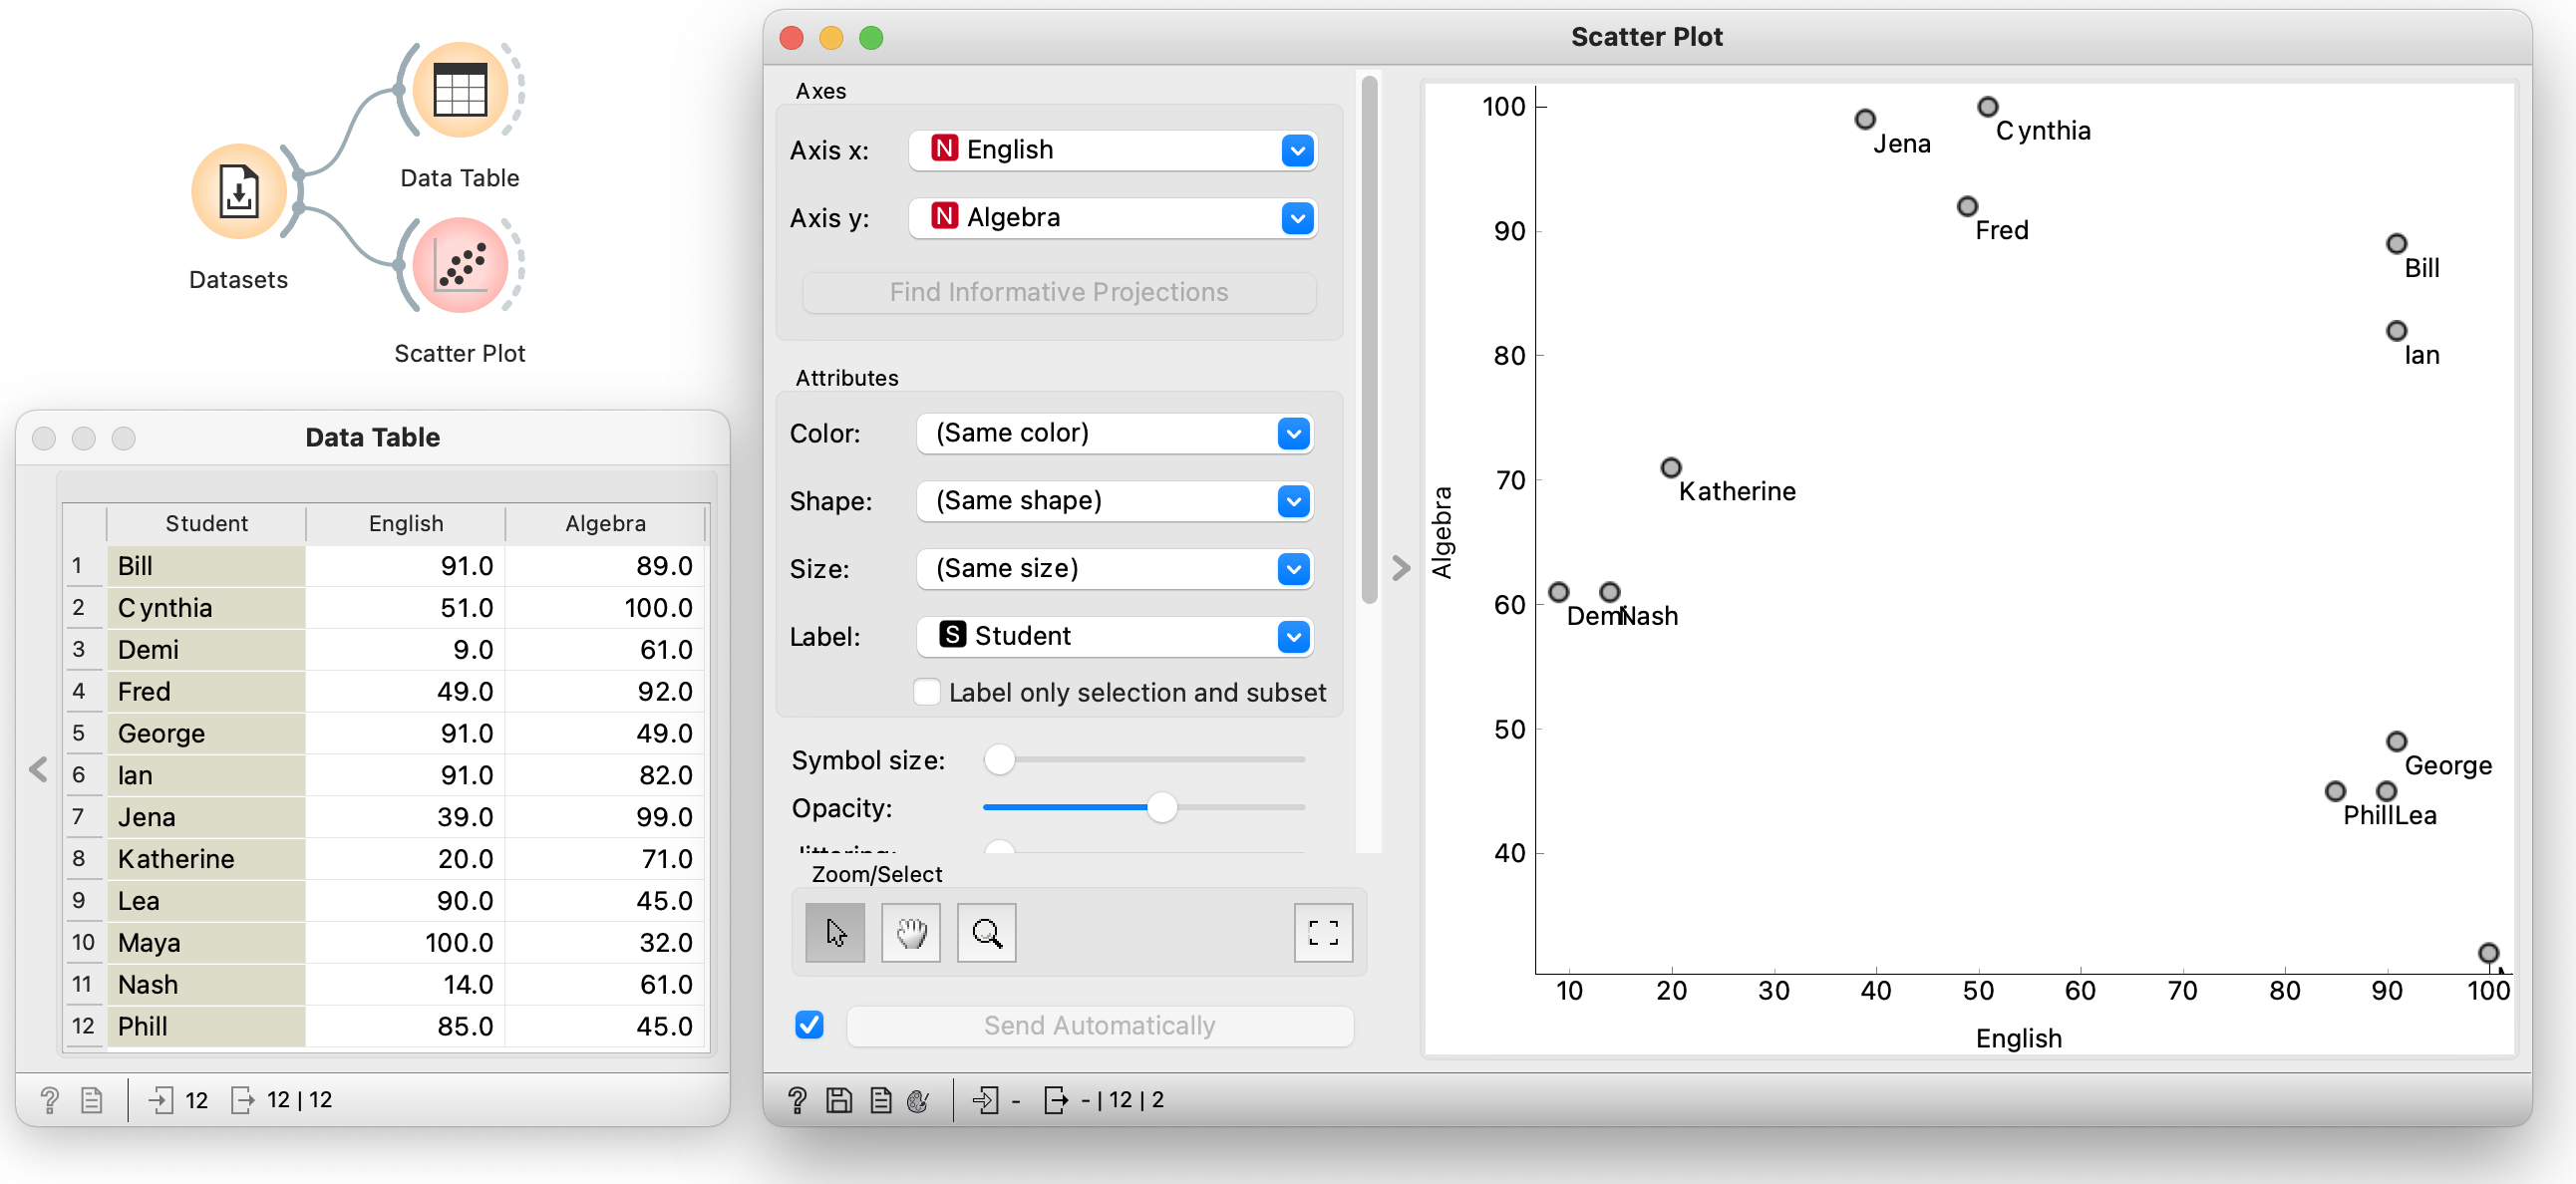
\includegraphics[width=\linewidth]{grades.png}%
    \caption{Razvščanje v skupine bomo predstavili s preprostimi podatki o študentih in njihovih ocenah pri angleščini in matematiki. Podatki so dostopni v Datasets widgetu.}
    \label{fig:010-grades-example}
\end{figure*}
  
Kaj sploh pomeni ``podobno''? Študenti so opisani s številskimi spremenljivkami, torej s ocenami pri predmetu. Ena od mer podobnosti je \textit{evklidska razdalja}, ki preprosto izmeri razdaljo med dvema študentoma (točkama) v prostoru, kot bi to storili z metrom.

\marginnote{Načinov merjenja razdalj med skupinami je več. Način, ki smo ga opisali, se imenuje \textit{povprečna razdalja (average linkage)}. Lahko bi računali tudi \textit{razdaljo med najbližjima točkama v skupini (single linkage)} ali pa med točkama, ki sta si \textit{najbolj oddaljeni (complete linkage).}}
Sedaj definirajmo še postopek za razvrščanje v skupine. Recimo, da začnemo z vsakim dokumentom v svoji skupini, nato pa v vsakem koraku združimo skupini, ki sta si najbolj podobni. Razdaljo med skupinami izračunamo kot povprečje razdalj med posameznimi elementi skupine. Tak postopek imenujemo hierarhično razvrščanje v skupine.

\newpage

Rezultate razvrščanja v skupine na primeru naših študentov si lahko pogledamo v sledečem delotoku:

\begin{marginfigure}[2cm]
    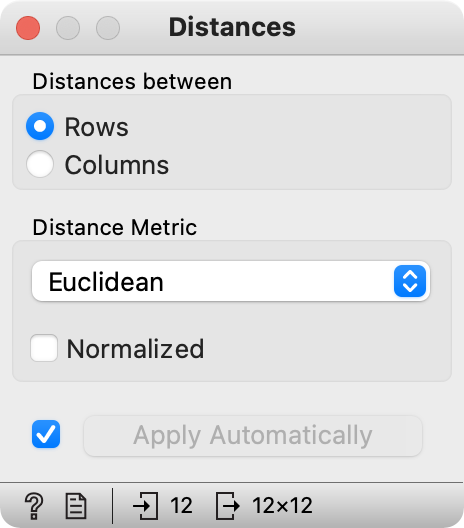
\includegraphics[width=\linewidth]{distances.png}
    \caption{}
\end{marginfigure}

\begin{figure}[h]
    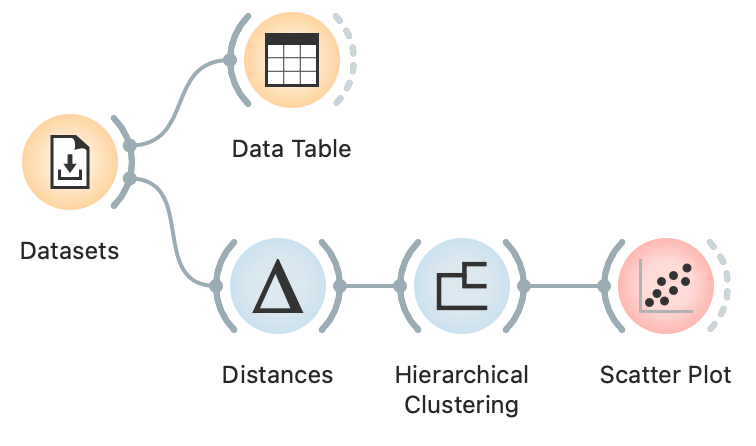
\includegraphics[width=\linewidth]{hierarchical-clustering-workflow.png}%
    \caption{ }
    \label{fig:010-hc-workflow}
\end{figure}

Naložite podatke z gradnikom \textit{Datasets}, izračunajte razdalje z gradnikom \textit{Distances}, uporabite \textit{Hierarchical Clustering} in si poglejte rezultate v gradniku \textit{Scatter Plot}. Gradnik Hierarchical Clustering omogoča, da hierarhijo skupin odrežemo pri določeni meri podobnosti in tako definiramo skupine.

\begin{figure*}[h]
    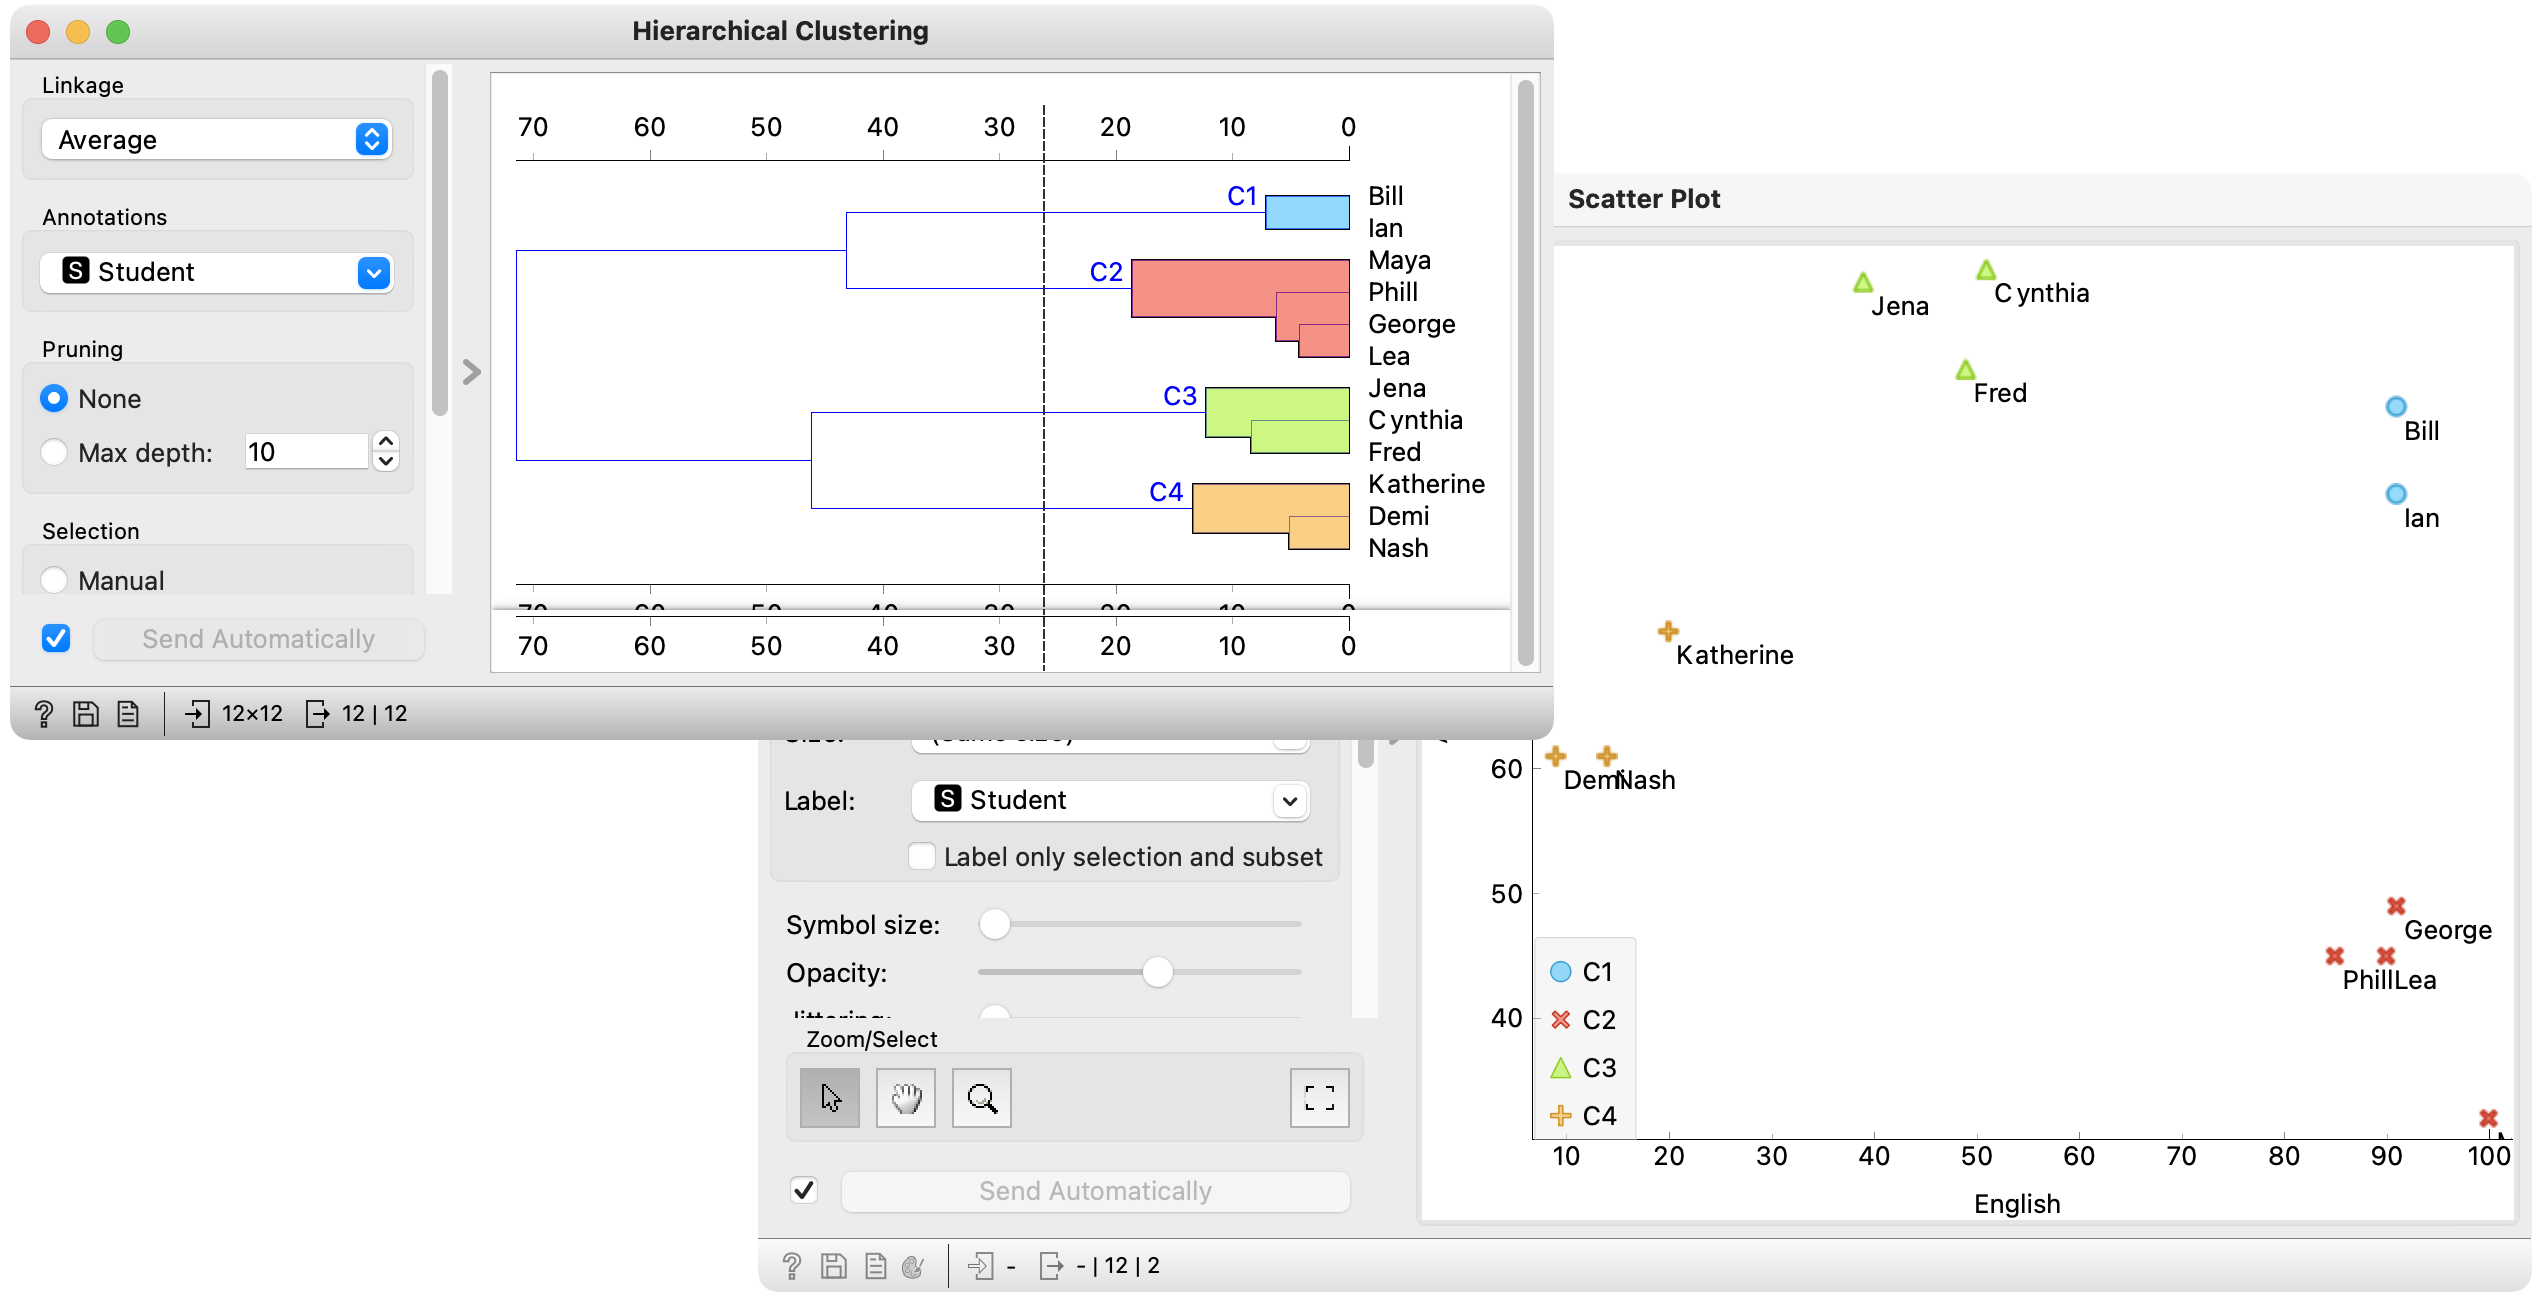
\includegraphics[width=\linewidth]{hc-scatter-plot.png}%
    \caption{ }
    \label{fig:010-hc-scatter-plot}
\end{figure*}